\section{Elektrobarošanas plates testi}
Testā tika novērtēts iekārtu jaudas patēriņš un elektrobarošanas risinājuma novērtējums.
\begin{figure}[H]
	\centering
    \includegraphics[width=0.9\textwidth]{pictures/test_diagram2.png}\hspace{1cm}
    \caption{9 un 5 V barošanas testa diagramma}
\end{figure}
3.9. att. redzams testa iekārtu slēgums elektriski principiālajā ķēdē un slodzes pieslēguma vieta.
\begin{table}[H]
\captionsetup{singlelinecheck=off, justification=raggedleft}
\caption{9 V elektrobarošanas}
\centering
\begin{tabular}{|c|c|c|c|c|c|}
\hline
\multicolumn{2}{|c|}{\makecell{Ieejas parametri}} 
& \multicolumn{2}{c|}{\makecell{Izejas parametri}} 
& \multirow{2}{*}{\makecell{Slodze, \si{\ohm}}} 
& \multirow{2}{*}{\makecell{Eff, \%}} \\
\cline{0-3}
\makecell{Spriegums, \si{\volt}} 
& \makecell{Strāva, \si{\ampere}}
& \makecell{Spriegums, \si{\volt}}
& \makecell{Strāva, \si{\ampere}}
&  &\\ 
\hline
12.04\pm0.12 & 0.02\pm0.01 & 8.95\pm0.01 & 0.01\pm0.00 & 14280.00\pm0.00 & 37.16 \\ 
\hline
12.06\pm0.12 & 0.12\pm0.01 & 8.96\pm0.01 & 0.10\pm0.00 & 90.14\pm0.00 & 61.91 \\ 
\hline
12.02\pm0.12 & 0.22\pm0.01 & 8.96\pm0.01 & 0.20\pm0.00 & 44.84\pm0.00 & 67.76 \\ 
\hline
12.03\pm0.12 & 0.32\pm0.02 & 8.98\pm0.01 & 0.30\pm0.00 & 29.90\pm0.00 & 69.98 \\ 
\hline
12.03\pm0.12 & 0.42\pm0.02 & 8.98\pm0.01 & 0.40\pm0.00 & 22.44\pm0.00 & 70.09 \\ 
\hline
12.00\pm0.12 & 0.53\pm0.02 & 8.99\pm0.01 & 0.50\pm0.00 & 17.96\pm0.00 & 70.68 \\ 
\hline
11.99\pm0.12 & 0.63\pm0.02 & 8.99\pm0.01 & 0.60\pm0.00 & 14.98\pm0.00 & 71.40 \\ 
\hline
11.98\pm0.12 & 0.73\pm0.02 & 9.00\pm0.01 & 0.70\pm0.00 & 12.85\pm0.00 & 72.04 \\ 
\hline
11.98\pm0.12 & 0.83\pm0.02 & 9.00\pm0.01 & 0.80\pm0.00 & 11.25\pm0.00 & 72.41 \\ 
\hline
11.97\pm0.12 & 0.93\pm0.03 & 9.00\pm0.01 & 0.90\pm0.00 & 10.01\pm0.00 & 72.76 \\ 
\hline
11.96\pm0.12 & 1.03\pm0.03 & 9.00\pm0.01 & 1.00\pm0.00 & 8.99\pm0.00 & 73.06 \\ 
\hline
\end{tabular}
\end{table}

Izveidotais 9 V pārveidotāja risinājums spēj nodrošināt nepieciešamo jaudu slodzei.

\begin{table}[H]
\centering
\captionsetup{singlelinecheck=off, justification=raggedleft}
\caption{5 V elektrobarošanas}
\begin{tabular}{|c|c|c|c|c|c|}
\hline
\multicolumn{2}{|c|}{\makecell{Ieejas parametri}} 
& \multicolumn{2}{c|}{\makecell{Izejas parametri}} 
& \multirow{2}{*}{\makecell{Slodze, \si{\ohm}}} 
& \multirow{2}{*}{\makecell{Eff, \%}} \\
\cline{0-3}
\makecell{Spriegums, \si{\volt}} 
& \makecell{Strāva, \si{\ampere}}
& \makecell{Spriegums, \si{\volt}}
& \makecell{Strāva, \si{\ampere}}
&  &\\ 
\hline
8.95\pm0.01 & 0.02\pm0.01 & 5.15\pm0.01 & 0.01\pm0.00 & 13020.00\pm0.00 &  28.61 \\ 
\hline
8.96\pm0.01 & 0.11\pm0.01 & 5.15\pm0.01 & 0.10\pm0.00 & 51.22\pm0.00 & 52.02 \\ 
\hline
8.96\pm0.01 & 0.21\pm0.01 & 5.16\pm0.01 & 0.20\pm0.00 & 25.70\pm0.00 & 54.50 \\ 
\hline
8.98\pm0.01 & 0.31\pm0.02 & 5.16\pm0.01 & 0.30\pm0.00 & 17.19\pm0.00 & 55.37 \\ 
\hline
8.98\pm0.01 & 0.41\pm0.02 & 5.16\pm0.01 & 0.40\pm0.00 & 12.89\pm0.00 & 56.10 \\ 
\hline
8.99\pm0.01 & 0.51\pm0.02 & 5.16\pm0.01 & 0.50\pm0.00 & 10.31\pm0.00 & 56.28 \\ 
\hline
8.99\pm0.01 & 0.61\pm0.02 & 5.16\pm0.01 & 0.60\pm0.00 & 8.59\pm0.00 & 56.42 \\ 
\hline
9.00\pm0.01 & 0.71\pm0.02 & 5.15\pm0.01 & 0.70\pm0.00 & 7.35\pm0.00 & 54.87 \\ 
\hline
9.00\pm0.01 & 0.81\pm0.02 & 5.14\pm0.01 & 0.80\pm0.00 & 6.43\pm0.00 & 56.52 \\ 
\hline
9.00\pm0.01 & 0.91\pm0.03 & 5.15\pm0.01 & 0.90\pm0.00 & 5.72\pm0.00 & 56.60 \\ 
\hline
9.00\pm0.01 & 1.01\pm0.03 & 5.15\pm0.01 & 1.00\pm0.00 & 5.14\pm0.00 & 56.66 \\ 
\hline
\end{tabular}
\end{table}

Izveidotais 5 V pārveidotāja risinājums spēj nodrošināt nepieciešamo jaudu slodzei. Slēdzot to kaskādes slēgumā pēc 9 V elektrobarošanas avota, tiek paaugstināta lineārā sprieguma efektivitāte, jo ir mazāk jaudas jāizkliedē uz sevis.

\begin{figure}[H]
\centering
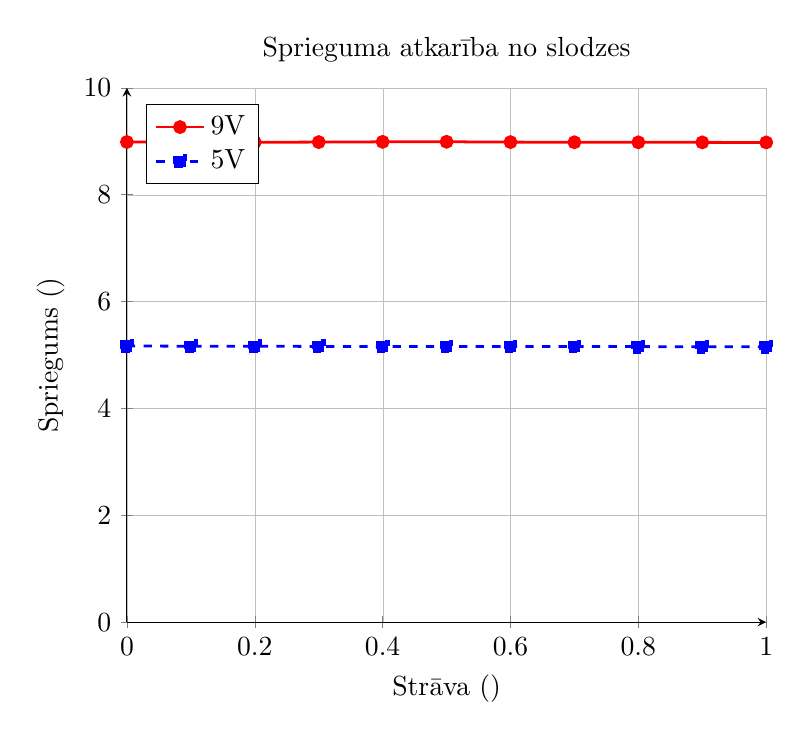
\begin{tikzpicture}
\begin{axis}[
    title={Sprieguma atkarība no slodzes},
    xlabel={Strāva (\si{\ampere})},
    ylabel={Spriegums (\si{\volt})},
    xmin=0, xmax=1,
    ymin=0, ymax=10,
    grid=both,
    grid style={line width=0.1pt, draw=gray!50},
    width=0.8\textwidth,
    axis lines=left,
    legend pos=north west,
]

% Line 1: 9V (Red)
\addplot[
    color=red,
    mark=*,
    line width=1pt,
]
coordinates {
    (0, 8.987)
    (0.1, 8.985)
    (0.2, 8.983)
    (0.3, 8.985)
    (0.4, 8.990)
    (0.5, 8.991)
    (0.6, 8.985)
    (0.7, 8.982)
    (0.8, 8.981)
    (0.9, 8.980)
    (1, 8.979)
};
\addlegendentry{9V}

% Line 2: 5V (Blue)
\addplot[
    color=blue,
    mark=square*,
    dashed,
    line width=1pt,
]
coordinates {
    (0, 5.168)
    (0.1, 5.165)
    (0.2, 5.163)
    (0.3, 5.161)
    (0.4, 5.160)
    (0.5, 5.160)
    (0.6, 5.159)
    (0.7, 5.158)
    (0.8, 5.157)
    (0.9, 5.155)
    (1, 5.153)
};
\addlegendentry{5V}

\end{axis}
\end{tikzpicture}
\caption{Strāvas-sprieguma raksturlīkne 9V un elektrobarošanas līnijām}
\end{figure}
Grafiski atveidoti iegūtie rezultāti. Maksimālais strāvas patēriņš 9 V līnijai ir 310 mA un 5 V līnijai 110 mA.